% This is "sig-alternate.tex" V2.1 April 2013
% This file should be compiled with V2.5 of "sig-alternate.cls" May 2012
%
% This example file demonstrates the use of the 'sig-alternate.cls'
% V2.5 LaTeX2e document class file. It is for those submitting
% articles to ACM Conference Proceedings WHO DO NOT WISH TO
% STRICTLY ADHERE TO THE SIGS (PUBS-BOARD-ENDORSED) STYLE.
% The 'sig-alternate.cls' file will produce a similar-looking,
% albeit, 'tighter' paper resulting in, invariably, fewer pages.
%
% ----------------------------------------------------------------------------------------------------------------
% This .tex file (and associated .cls V2.5) produces:
%       1) The Permission Statement
%       2) The Conference (location) Info information
%       3) The Copyright Line with ACM data
%       4) NO page numbers
%
% as against the acm_proc_article-sp.cls file which
% DOES NOT produce 1) thru' 3) above.
%
% Using 'sig-alternate.cls' you have control, however, from within
% the source .tex file, over both the CopyrightYear
% (defaulted to 200X) and the ACM Copyright Data
% (defaulted to X-XXXXX-XX-X/XX/XX).
% e.g.
% \CopyrightYear{2007} will cause 2007 to appear in the copyright line.
% \crdata{0-12345-67-8/90/12} will cause 0-12345-67-8/90/12 to appear in the copyright line.
%
% ---------------------------------------------------------------------------------------------------------------
% This .tex source is an example which *does* use
% the .bib file (from which the .bbl file % is produced).
% REMEMBER HOWEVER: After having produced the .bbl file,
% and prior to final submission, you *NEED* to 'insert'
% your .bbl file into your source .tex file so as to provide
% ONE 'self-contained' source file.
%
% ================= IF YOU HAVE QUESTIONS =======================
% Questions regarding the SIGS styles, SIGS policies and
% procedures, Conferences etc. should be sent to
% Adrienne Griscti (griscti@acm.org)
%
% Technical questions _only_ to
% Gerald Murray (murray@hq.acm.org)
% ===============================================================
%
% For tracking purposes - this is V2.0 - May 2012

\documentclass{sig-alternate-05-2015}

\def\sharedaffiliation{%
\end{tabular}
\begin{tabular}{c}}

\usepackage{hyperref}
\begin{document}

% Copyright
%\setcopyright{acmcopyright}
%\setcopyright{acmlicensed}
%\setcopyright{rightsretained}
%\setcopyright{usgov}
%\setcopyright{usgovmixed}
%\setcopyright{cagov}
%\setcopyright{cagovmixed}

% DOI
%\doi{10.475/123_4}

% ISBN
%\isbn{123-4567-24-567/08/06}

%Conference
%\conferenceinfo{PLDI '13}{June 16--19, 2013, Seattle, WA, USA}

%\acmPrice{\$15.00}

%
% --- Author Metadata here ---
%\conferenceinfo{WOODSTOCK}{'97 El Paso, Texas USA}
%\CopyrightYear{2007} % Allows default copyright year (20XX) to be over-ridden - IF NEED BE.
%\crdata{0-12345-67-8/90/01}  % Allows default copyright data (0-89791-88-6/97/05) to be over-ridden - IF NEED BE.
% --- End of Author Metadata ---

\title{Smart Stylus (aka Air Doodle)}
\subtitle{EECS 149/249A Class Project}
% \title{Alternate {\ttlit ACM} SIG Proceedings Paper in LaTeX
% Format\titlenote{(Produces the permission block, and
% copyright information). For use with
% SIG-ALTERNATE.CLS. Supported by ACM.}}
%\subtitle{[Extended Abstract]
%\titlenote{A full version of this paper is available as
%\textit{Author's Guide to Preparing ACM SIG Proceedings Using
%\LaTeX$2_\epsilon$\ and BibTeX} at
%\texttt{www.acm.org/eaddress.htm}}}
%
% You need the command \numberofauthors to handle the 'placement
% and alignment' of the authors beneath the title.
%
% For aesthetic reasons, we recommend 'three authors at a time'
% i.e. three 'name/affiliation blocks' be placed beneath the title.
%
% NOTE: You are NOT restricted in how many 'rows' of
% "name/affiliations" may appear. We just ask that you restrict
% the number of 'columns' to three.
%
% Because of the available 'opening page real-estate'
% we ask you to refrain from putting more than six authors
% (two rows with three columns) beneath the article title.
% More than six makes the first-page appear very cluttered indeed.
%
% Use the \alignauthor commands to handle the names
% and affiliations for an 'aesthetic maximum' of six authors.
% Add names, affiliations, addresses for
% the seventh etc. author(s) as the argument for the
% \additionalauthors command.
% These 'additional authors' will be output/set for you
% without further effort on your part as the last section in
% the body of your article BEFORE References or any Appendices.

\numberofauthors{3} %  in this sample file, there are a *total*
% of EIGHT authors. SIX appear on the 'first-page' (for formatting
% reasons) and the remaining two appear in the \additionalauthors section.
%
\author{
% You can go ahead and credit any number of authors here,
% e.g. one 'row of three' or two rows (consisting of one row of three
% and a second row of one, two or three).
%
% The command \alignauthor (no curly braces needed) should
% precede each author name, affiliation/snail-mail address and
% e-mail address. Additionally, tag each line of
% affiliation/address with \affaddr, and tag the
% e-mail address with \email.
%
% 1st. author
%\alignauthor
%\titlenote{Dr.~Trovato insisted his name be first.}\\
%       \affaddr{Institute for Clarity in Documentation}\\
%       \affaddr{1932 Wallamaloo Lane}\\
%       \affaddr{Wallamaloo, New Zealand}\\
%       \email{trovato@corporation.com}
%% 2nd. author
%\alignauthor
%G.K.M. Tobin\titlenote{The secretary disavows
%any knowledge of this author's actions.}\\
%       \affaddr{Institute for Clarity in Documentation}\\
%       \affaddr{P.O. Box 1212}\\
%       \affaddr{Dublin, Ohio 43017-6221}\\
%       \email{webmaster@marysville-ohio.com}
%% 3rd. author
%\alignauthor Lars Th{\o}rv{\"a}ld\titlenote{This author is the
%one who did all the really hard work.}\\
%       \affaddr{The Th{\o}rv{\"a}ld Group}\\
%       \affaddr{1 Th{\o}rv{\"a}ld Circle}\\
%       \affaddr{Hekla, Iceland}\\
%       \email{larst@affiliation.org}
%\and  % use '\and' if you need 'another row' of author names
%% 4th. author
%\alignauthor Lawrence P. Leipuner\\
%       \affaddr{Brookhaven Laboratories}\\
%       \affaddr{Brookhaven National Lab}\\
%       \affaddr{P.O. Box 5000}\\
%       \email{lleipuner@researchlabs.org}
%% 5th. author
%\alignauthor Sean Fogarty\\
%       \affaddr{NASA Ames Research Center}\\
%       \affaddr{Moffett Field}\\
%       \affaddr{California 94035}\\
%       \email{fogartys@amesres.org}
%% 6th. author
%\alignauthor Charles Palmer\\
%       \affaddr{Palmer Research Laboratories}\\
%       \affaddr{8600 Datapoint Drive}\\
%       \affaddr{San Antonio, Texas 78229}\\
%       \email{cpalmer@prl.com}
%}
% 1st. author
\alignauthor
Mitchell Oleson \\
\email{moleson21@berkeley.edu} \\
% 2nd. author
\alignauthor
William Smith \\
\email{williampsmith@berkeley.edu} \\
% 3rd. author
%\and  % use '\and' if you need 'another row' of author names
\alignauthor
Gera Groshev \\
\email{groshevg@berkeley.edu} \\
% 4th. author
\sharedaffiliation
%\email{[antonio, marten, eal, alberto]@eecs.berkeley.edu} \\
\affaddr{Department of Electrical Engineering and Computer Science} \\
\affaddr{University of California}\\
\affaddr{Berkeley, CA} \\
}

% There's nothing stopping you putting the seventh, eighth, etc.
% author on the opening page (as the 'third row') but we ask,
% for aesthetic reasons that you place these 'additional authors'
% in the \additional authors block, viz.
% \additionalauthors{Additional authors: John Smith (The Th{\o}rv{\"a}ld Group,
% email: {\texttt{jsmith@affiliation.org}}) and Julius P.~Kumquat
% (The Kumquat Consortium, email: {\texttt{jpkumquat@consortium.net}}).}
% \date{30 July 1999}
% Just remember to make sure that the TOTAL number of authors
% is the number that will appear on the first page PLUS the
% number that will appear in the \additionalauthors section.

\maketitle
\begin{abstract}
Modern human computer interaction has increasingly gone in the direction of control via intuitive physical gestures. These increasingly rely on sensor data, and are therefore suitable for embedded platforms. In this respect, we detail a prototype implementation of a glove device that recognizes hand gestures and uses these to drive an LED Matrix. We discuss system architecture, algorithm design, implementation choices, and analysis of the results on a chosen set of character gestures.
\end{abstract}


%
% The code below should be generated by the tool at
% http://dl.acm.org/ccs.cfm
% Please copy and paste the code instead of the example below. 
%
% \begin{CCSXML}
% <ccs2012>
%  <concept>
%   <concept_id>10010520.10010553.10010562</concept_id>
%   <concept_desc>Computer systems organization~Embedded systems</concept_desc>
%   <concept_significance>500</concept_significance>
%  </concept>
%  <concept>
%   <concept_id>10010520.10010575.10010755</concept_id>
%   <concept_desc>Computer systems organization~Redundancy</concept_desc>
%   <concept_significance>300</concept_significance>
%  </concept>
%  <concept>
%   <concept_id>10010520.10010553.10010554</concept_id>
%   <concept_desc>Computer systems organization~Robotics</concept_desc>
%   <concept_significance>100</concept_significance>
%  </concept>
%  <concept>
%   <concept_id>10003033.10003083.10003095</concept_id>
%   <concept_desc>Networks~Network reliability</concept_desc>
%   <concept_significance>100</concept_significance>
%  </concept>
% </ccs2012>  
% \end{CCSXML}

% \ccsdesc[500]{Computer systems organization~Embedded systems}
% \ccsdesc[300]{Computer systems organization~Redundancy}
% \ccsdesc{Computer systems organization~Robotics}
% \ccsdesc[100]{Networks~Network reliability}


%
% End generated code
%

%
%  Use this command to print the description
%
% \printccsdesc

% We no longer use \terms command
%\terms{Theory}

% \keywords{ACM proceedings; \LaTeX; text tagging}

\section{Introduction}
Due to the recent rise of wearables, mobile devices, and the Internet of Things, there has been a great deal of recent interest in using embedded and mobile devices in order to recognize gestures. For example, using smart watches to classify exercises is currently  an active area of research [1]. Our objective was to prototype our own embedded device platform both for sensing of user movement and classification of the associated gestures. We wanted the platform to be general, so that it could support a wide variety of uses, such as virtual design, human computer interaction, remote control of devices and movement classification. We therefore devised a glove system that uses 2 Raspberry Pi Microcontrollers, networked via bluetooth, one affixed to the glove, and decided to demonstrate a particular use case, namely, actuating an LED matrix. The glove device is wireless, includes an accelerometer, gyroscope, and magnetometer, and has enough local computational resources to support time-series machine learning classification algorithms. It performs classification locally, and then wirelessly transmits a byte, or several bytes, to a remote system which contains a library of gestures. It therefore allows for a very wide variety of gesture recognition applications, and is both lightweight and powerful. We chose to demonstrate and test ours on a simple subset of digits drawn in midair using the device. The following report details our design, implementation, and analysis.

\section{Hardware Architecture}

\begin{figure*}
\centering
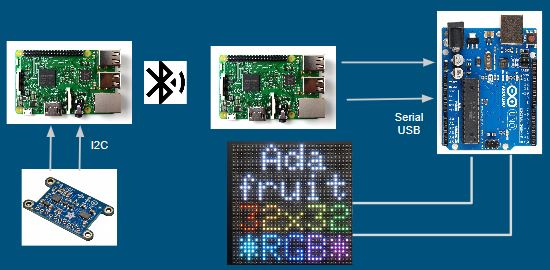
\includegraphics{figure0}
\caption{Image detailing the interfaces and connections between each of the hardware aspects.}
\end{figure*}

The Adafruit BNO055 Absolute Orientation Sensor is a breakout board for the surface mounted BNO055 Sensor. It provides a convenient connection to the surface mounted chip via an I$^2$C interface and allows direct read write capabilities to the internal registers. These registers house absolute orientation (both euler and quaternion form), angular velocity, acceleration (gravity+linear motion), linear accel (linear motion), gravity, magnetic field strength, and temperature. In order to accomplish this multitude of readings on a single device, the BNO055 uses onboard hardware (and software) sensor fusion. This allowed us to get up and running with pure motion acceleration from a reliable source for training the gesture recognition model. To interface with the I$^2$C line we had initially used an Arduino with Adafruit`s provided libraries [1] for the final project however, we used a Raspberry Pi 3.

The Raspberry Pi 3 is a micro computer toting a 1.2GHz 64-bit quad-core ARMv8 CPU with onboard 802.11n Wireless LAN, Bluetooth 4.1 (including BLE), and a 40 pin GPIO header at a cost of \$35 each. These features made it an ideal candidate for our project as we need one reading the sensor and another sending the commands to the Arduino for the LED Matrix. We utilized the onboard Bluetooth 4.1 and the linux bluetooth-dev libraries to setup a connection between the two Pi`s. Furthermore, the 40 pin GPIO header made it easy to setup buttons using WiringPi [2] for both interrupt control (data collection via button press and hold) and the glove LED to provide visual feedback during data collection. Finally, we used the GPIO headers I$^2$C connection to talk between the sensor and Pi on the glove device and the USB connection on the second Pi to talk with the Arduino to control the LED Matrix. To talk with the sensor over I$^2$C, we translated the sensors Arduino C code written by Adafruit [1] to read and write over the Pi`'s I$^2$C pins. In addition, due to a hardware bug with the I$^2$C Master on the BCM2835 [3], the Raspberry Pi cannot do arbitrary clock stretching (phenomena when the I$^2$C slave slows down communication by holding SCL low to synchronize clocks and/or process requests) which the BNO055 did regularly causing complete data corruption. To overcome the bug without switching sensors (which would`ve started us back at square one), we manually set the I$^2$C baud rate to more than the maximum stretch time. Essentially, what we did is slow down our communication speed to account for the longer clock cycles. This means that we aren`'t able to read/write as fast as we normally would (decreased from 100KHz default to 50KHz), however, since we are only communicating with a single sensor and don`t' constantly poll (only want every 50ms), there is no noticeable difference. For more information about this hardware bug checkout: \url{http://elinux.org/BCM2835_datasheet_errata#p35_I2C_clock_stretching}.

\section{Software Architecture}

\subsection{Data Collection \& Classification Pipeline}
The glove device consisted of a multithreaded C++ application running on the Raspberry Pi 3 that waits for an interrupt (button press) before turning on an LED and generating a time series matrix of polled sensor data. This matrix is generated live by reading the BNO055`s Linear Acceleration data registers (registers 0x28 to 0x2D) over I$^2$C while the button is held. Once the button is released, we would exit out of the polling loop and split off into a new thread for classification and transmission. By creating a new thread we allowed the main program to continue on and wait for the next interrupt for drawing gestures regardless of classification and/or transmission lag. To ensure this threaded structure was safe, we made use of three mutexes: newData, threads, and blue. The newData mutex was acquired at the start of data collection with its primary purpose to aid in button debouncing and ensure that only one thread was ever reading sensor data and creating a new data time series. When coupled with a matrix size check at the end of polling, we were able to successfully debounce the button and ensure that only one data set is generated per button press. The second mutex, threads, was used to preserve ordering of the written gestures across to the multiple threads and the two asynchronous Raspberry Pi`s as well as the number of active threads. It was particularly important to keep track of thread ordering as it wasn`t guaranteed that the transmission order would match the original drawn order. This is a result of the classification step prior to sending that can take an arbitrary amount of time before completing making it possible for rapid gestures to classify and send out of order. The second purpose of the threads mutex is to track the number of currently processing threads. This is key when we wish to exit out of the program (which is made possibly by polling a button in the main function loop). If we were to exit out prematurely it would cause the system to mark relevant data as trash and remove it from memory. To ensure this doesn`'t happen, we first acquire the newData mutex thus preventing new threads from spawning then wait till the aliveThreads variable is equal to zero (i.e. no threads running). Once this check is passed we acquire the blue mutex to send an end message before gracefully closing the bluetooth socket and exiting the program. The final mutex, blue, must be acquired before sending anything across the bluetooth interface. This is probably the most straightforward of the mutexes as only one thread is allowed to be sending something at a time otherwise errors or data corruption might occur.

\subsection{Display Pipeline}
For the matrix control side, we utilized the second Pi running a single threaded python program to continuously poll then display the transmitted bluetooth data. Essentially, this Pi was set up as the bluetooth server and awaited data to come across the connection to the glove device. Once received, it checked that it wasn`t an end message before parsing the data in 3 byte chunks (threadNum, gesture, likelihood). It would then check for equality between the parsed threadNum and its own curr variable (which was synced to the next expected display gesture). If these two happened to be unequal, it would add the gesture to a dictionary with the corresponding threadNum as its key. We would then continue parsing data or go back to receiving until the curr equality was satisfied (meaning that we had the correct next gesture). Once it was satisfied we transmit a bitmap corresponding to the classified gesture to the Arduino via USB before incrementing the curr counter to the next expected value. Once incremented, the program checks the dictionary to see if the new curr value is present and if it is, updates and sends a new bitmap to the Arduino for display.

\subsection{LED Matrix}
We used the 32x32 RGB LED Matrix Panel sold by Adafruit Industries [6] and controlled it with the Arduino. To do this, the Arduino received 128 bytes via serial COM, which was sent from a Raspberry Pi using PySerial [8] to transmit via Python, and stored them in a 128 element array. Each byte represented 8 bits of a 32x32 bit bitmap. The bits represented whether a LED pixel was on or off and were read in left to right, top to bottom order. To display the bitmap we used the Adafruit\_GFX [6] and RGBmatrixPanel [6] libraries. First we cleared the screen with the fillScreen() method, sending in a color code of (0,0,0), then we used the drawBitmap() method to display the 128 byte bitmap. Once the bitmap was displayed, the display latched and the Arduino was set to wait in a loop until another sequence of 128 bytes was available to overwrite the bitmap.

\section{Algorithms}
One of the core drivers of accomplishing the goal of real time gesture recognition exists in finding a suitable classification algorithm. This algorithm needed to consist of a lightweight and non-computationally intensive model, suitable for storage and running on an embedded platform. Additionally, the algorithm should be robust enough to handle differences in speed and duration of a gesture, but also capable of identifying the relative ordering of a gesture sequence. We first evaluated the feasibility of generating bitmaps of the traced shape, and then performing optical character recognition. This required the use of dead reckoning in order to convert the raw accelerometer data.

\subsection{Dead Reckoning}

\begin{figure}
\centering
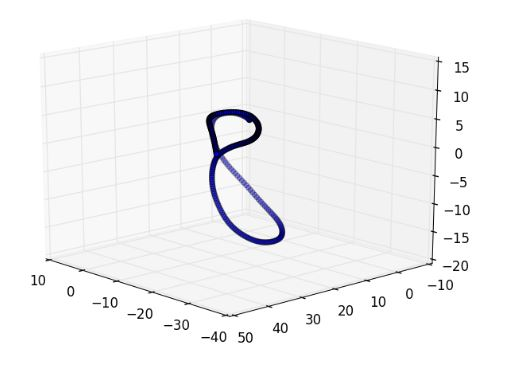
\includegraphics[height=1in, width=1in]{figure1}
\caption{Bitmap Ouput of Figure 8 from Dead Reckoning}
\vskip -6pt
\end{figure}

In the prototyping phase, we utilized the Wiimote in order to take in x, y, and z acceleration, as well as pitch and roll, using the code generated in lab. This data was calibrated and offset, as well as passed through a moving average filter, to make it suitable for prototyping data. We collected data for tracing the 10 digits in air. Our algorithm consisted of the following parts: We begin by computing the nominal gravity vector, by averaging the first 10 samples. This therefore assumes that the user allows for a brief  position of non-movement in the beginning of the sample. We then remove the gravity vector from all vectors in the sample. This assumes that the gravity vector does not change much throughout the movement, which is an acceptable assumption since the movement is planar. We next perform trapezoidal integration on acceleration, in order to obtain velocity, and then again to obtain position. Finally, we perform Singular Value Decomposition on the resultant matrix, and principal component analysis. This factors the position matrix into the product of 3 matrices, which allow us to deduce the principal components of the data and their magnitude. The purpose of this was to create a 2 dimensional bitmap from 3D data, invariant  of rotation. We then project the position matrix into this 2D space.

\begin{figure}
\centering
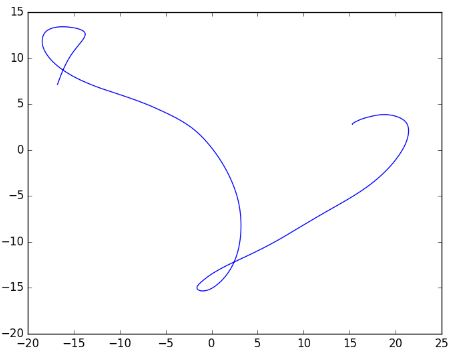
\includegraphics[height=1in, width=1in]{figure2}
\caption{Ouput of SVD/PCA Showing Y Drift}
\vskip -6pt
\end{figure}

Running this algorithm, however, the cumulative error from the double integration was apparent when looking at the data, which quickly asymptoted to large values. We therefore decided to use kinematic equations, specifically $d = d0 + vt + \frac{1}{2}at^2$. This showed a dramatic improvement. Figure (2) shows the results of generating bitmaps using this algorithm. However, we noticed that the y axis exhibited a drift. This was being caused by an un-accounted for nonzero constant bias in the y acceleration, which accumulated over time when converting to position. The drift was significant, and caused singular value decomposition to project into the wrong plane (since we project into the plan of maximum variance). Since we ultimately do not need this axis, we decided to throw out the y data altogether. We later changed the input of this algorithm to the BNO055 sensor accel data. However, the sensor has hardware support for removing gravity and calibration, so we exploited these.

\subsection{Gesture Recognition}
Originally, the purpose of creating bitmaps of the position trace was to perform optical character recognition on the resultant bitmap. This allowed us to use well used and well researched algorithms, such as Convolutional Neural Networks or Nearest Neighbor, and well publicized training datasets, such as MNIST  [4]. In addition, the bitmap, after resizing, would be suitable as an input to the LED Matrix control. However, we realized that there were several disadvantages in using a static bitmap, as opposed to time varying data. For example, using time-varying data would allow a more general form of gesture recognition. For example, a `swipe left` gesture and `swipe right` gesture would look the same once mapped to a position bitmap. However, a time series dataset would show a change of position in the position x direction for the case of a `swipe right` gesture, as opposed to an initial change in the negative x direction for a `swipe left`. This same idea can be used to make the device suitable for arbitrary gestures. We therefore chose to use an algorithm known as Dynamic Time Warping (henceforth, DTW). DTW is a lightweight, unsupervised machine learning algorithm used for comparing multidimensional time-series data. During the training phase, the algorithm computes a canonical sequence for each classification label given example data. This sequence is the result of minimizing a loss function which computes the cumulative distance traveled on a path between the canonical sequence and the training example, at each point. This is done for each dimension of the signal. The algorithm transforms its canonical representation by stretching or skewing about the time axis to minimize this loss function. During testing and classification, the test example is compared to each canonical signal (there is one per classification label. In the case of classifying the digits, there will be 10 such signals). The loss function is computed, and the classification is chosen as the argmax, i.e., the class mabel that minimizes the loss function. This is output with an associated maximum likelihood, thereby allowing the algorithm to choose no classification in the case where the gesture is not close to any example. Real time classification of DTW runs in O(NM) runtime, where M represents the length of the longest canonical sequence, and N represents the length of the sequence to be classified [5]. It is therefore relatively fast compared to a neural network, making it suitable for embedded devices. Because the model can be trained on any machine, and deployed and ran on another device with only the saved canonical signals, it is low in memory requirements (O(kM) space complexity).  For the purpose of designing this classification pipeline, we chose to use the Gesture Recognition Toolkit  [7].

The gesture recognition toolkit supports training a pipeline, which consists of a classification algorithm (in our case, DTW), pre-processing algorithms, and post-processing. Our implementation consisted of two pre-processing algorithms, in order to remain consistent with the implementation of the prototype data using the WiiMote. We chose to use a moving average filter for preprocessing, and a thresholding trim algorithm, wherein all datapoints below a certain energy threshold are removed, where the energy threshold is given as a percentage if the maximum energy of the time-series. We tried two different data streams for training the algorithm. The first was the conditioned (gravity removed, calibrated and bias offset) x and z acceleration. We trained these on the gestures 0, 8, and 9, and obtained positive results (70\% + on average, over multiple training instances, with an upper bound of 93\%). However, when we trained using multiple user input, we noticed lesser results. We found that the reason for this was differences in the speed of the gesture between users, which can cause differences in signal amplitude, a metric that affects the loss function dramatically. Next, we tried the position data obtained by running the data through our dead reckoning algorithm as an additional pre-processing step. This yielded results in excess of 93\% consistently.

\section{Conclusions}
Much work can still be done in order to improve this system. Due to the data intensive nature of machine learning algorithms, we were not able to classify a wide variety of gestures, however we would like to further demonstrate this model on arbitrary gestures such as left and right swipes, and all of the letters of the alphabet. One possible improvement of the device would be to add support for real-time update of the learning model so that the device can adjust to the gesture pattern of the individual user. We would like to generate and control animations in order to use the platform more interactively. Possible uses for such a device that we envision include entertainment system control, interactive art and design via physical manipulation of digital illustration, and quick real-time control of large scale displays, such as at a sporting event.
%\end{document}  % This is where a 'short' article might terminate

%ACKNOWLEDGMENTS are optional
\section{References}
[1] Adafruit\_BNO055 Unified Sensor Library (https://github\newline .com/adafruit/Adafruit\_BNO055) written by Kevin Townsend for Adafruit Industries
\newline
\newline
[2] WiringPi (http://wiringpi.com/) written by Gordon Henderson
\newline
\newline
[3] BCM2835 Errata Datasheet (http://elinux.org/BCM2835\newline \_datasheet\_errata) written by Elinux
\newline
\newline
[4] MNIST Database of Handwritten Digits (http://yann.lecun.com\newline /exdb/mnist/)
\newline
\newline
[5] Muller, M. Information Retrieval for Music and Motion (http://www.springer.com/cda/content/document/cda\_\newline gdownloaddocument/9783540740476-c1.pdf?SGWID=0-0-45-452103-p173751818)
\newline
\newline
[6] Adafruit-GFX-Library (https://github.com/adafruit/Adafruit-GFX-Library) and RGB-matrix-Panel (\url{https://github.com/adafruit/RGB-matrix-Panel}) are libraries written by Limor Fried and Phil Burgess for Adafruit Industries. Copyright (c) 2012 Adafruit Industries. All rights reserved. Distributed under the BSD license.
\newline
\newline
[7] The source code for the Arduino software in the Java environment is released under the GPL license and the C/C++ microcontroller libraries are under the LGPL license.
\newline
\newline
[8] PySerial, created by Chris Liechti, is distributed under the BSD license. Copyright (c) 2001-2015 Chris Liechti <cliechti@gmx.net>. All Rights Reserved.
\newline
\newline
[9] NumPy libraries started by Travis Oliphant. Copyright © 2005-2016, NumPy Developers. All rights reserved. Distributed under the BSD license.
\newline
\newline
[10] Matplotlib libraries created by John Hunter. Copyright (c) 2012-2013 Matplotlib Development Team. All Rights Reserved. License based on Python Software Foundation (PSF) license.
\newline
\newline


%
% The following two commands are all you need in the
% initial runs of your .tex file to
% produce the bibliography for the citations in your paper.
%\bibliographystyle{abbrv}
%\bibliography{sigproc}  % sigproc.bib is the name of the Bibliography in this case
% You must have a proper ".bib" file
%  and remember to run:
% latex bibtex latex latex
% to resolve all references
%
% ACM needs 'a single self-contained file'!
%
%APPENDICES are optional
%\balancecolumns
\end{document}